\newpage
\section{Application to Fusion Simulation Data}
\label{sec:xgc}
We report on our application of the skinny matrix version to fusion
simulation data from the XGC code \cite{??}. The resulting data has
480 time steps, each with 32 equispaced polloidal slices. We perform 4
PCA decompositions of density potential ``dpot'' indexed by time steps
100, 200, 300, and 400, by taking the index time step and 15 more
following it to get a total of $32\times 16$ slices, each with 232,011
gridpoints. This results in a $256\times 232,011$ matrix, which is
very skinny and takes roughly 1 GB memory.

The decision to construct the PCA input matrix as described is
motivated by the need to view its rows as sample points from a
stationary distribution. It is reasonable to assume that the slices in
a single time step are from the same high dimensional (specifically,
232,011 dimensional) distribution that can be characterized by its top
principal components. Because our row dimension includes both time and
space (toroidal angle), there is a relationship between this
``stacked'' matrix PCA decomposition and the three dimensional tensor
decomposition. We describe some initial tensor decomposition results
for a similar data set in a subsection that follows.

Our algorithm is implemented in R with pbdR infrastructure
\cite{Schmidt2017}, which for the specific skinny matrix computations
utilizes MPI, LAPACK, and ADIOS library support. Our runs on OLCF
Rhea, which is a 512 node commodity cluster with dual Intel® Xeon®
E5-2650 @ 2.0 GHz giving 16 cores per node. Our runs are on 8 nodes
(128 cores) and take approximately 6 to 8 seconds to read the data
from a lustre file system, and under 2 seconds to perform the
decomposition. Production of 512 resulting plots of right singular
vectors and scree plots, like those shown in Figures~\ref{fig:100} to
\ref{fig:400}, takes roughly 100 seconds.

We expect that the resulting speeds are more than sufficient to keep
up with a running XGC simulation, which takes roughly four seconds per
time step \cite{XGCpertimestep}, giving 64 seconds for our 16 step
ensemble. We envision the decomposition code running as a service
connected to an ADIOS in memory staging file system. Next we comment
on the results in Figures~\ref{fig:100} to \ref{fig:400}.
\begin{figure}[tbp]
  \begin{center}
    \slc{0.245}{Figs/p100/pc00001.00100.png}
    \slc{0.245}{Figs/p100/pc00002.00100.png}
    \slc{0.245}{Figs/p100/pc00003.00100.png}
    \slc{0.245}{Figs/p100/pc00004.00100.png}\\
    \slc{0.245}{Figs/p100/pc00005.00100.png}
    \slc{0.245}{Figs/p100/pc00006.00100.png}
    \slc{0.245}{Figs/p100/pc00007.00100.png}
    \slc{0.245}{Figs/p100/pc00008.00100.png}\\
    \slc{0.245}{Figs/p100/pc00009.00100.png}
    \slc{0.245}{Figs/p100/pc00010.00100.png}
    \slc{0.245}{Figs/p100/pc00011.00100.png}
    \slc{0.245}{Figs/p100/pc00012.00100.png}\\
    \slc{0.245}{Figs/p100/pc00013.00100.png}
    \slc{0.245}{Figs/p100/pc00014.00100.png}
    \slc{0.245}{Figs/p100/pc00015.00100.png}
    \slc{0.245}{Figs/p100/pc00016.00100.png}\\
    \slc{0.245}{Figs/p100/pc00017.00100.png}
    \slc{0.245}{Figs/p100/pc00018.00100.png}
    \slc{0.245}{Figs/p100/pc00019.00100.png}
    \slc{0.245}{Figs/p100/pc00020.00100.png}\\
    \slc{0.245}{Figs/p100/pc00021.00100.png}
    \slc{0.245}{Figs/p100/pc00022.00100.png}
    \slc{0.245}{Figs/p100/pc00023.00100.png}
    \slc{0.245}{Figs/p100/pc00024.00100.png}\\
    \scr{0.35}{Figs/p100/scree.pdf}
    \scr{0.35}{Figs/p100/scree100log.pdf}
  \end{center}
  \caption{Time steps 100 to 115}
  \label{fig:100}
\end{figure}

\begin{figure}[tbp]
  \begin{center}
    \slc{0.245}{Figs/p200/pc00001.00200.png}
    \slc{0.245}{Figs/p200/pc00002.00200.png}
    \slc{0.245}{Figs/p200/pc00003.00200.png}
    \slc{0.245}{Figs/p200/pc00004.00200.png}\\
    \slc{0.245}{Figs/p200/pc00005.00200.png}
    \slc{0.245}{Figs/p200/pc00006.00200.png}
    \slc{0.245}{Figs/p200/pc00007.00200.png}
    \slc{0.245}{Figs/p200/pc00008.00200.png}\\
    \slc{0.245}{Figs/p200/pc00009.00200.png}
    \slc{0.245}{Figs/p200/pc00010.00200.png}
    \slc{0.245}{Figs/p200/pc00011.00200.png}
    \slc{0.245}{Figs/p200/pc00012.00200.png}\\
    \slc{0.245}{Figs/p200/pc00013.00200.png}
    \slc{0.245}{Figs/p200/pc00014.00200.png}
    \slc{0.245}{Figs/p200/pc00015.00200.png}
    \slc{0.245}{Figs/p200/pc00016.00200.png}\\
    \slc{0.245}{Figs/p200/pc00017.00200.png}
    \slc{0.245}{Figs/p200/pc00018.00200.png}
    \slc{0.245}{Figs/p200/pc00019.00200.png}
    \slc{0.245}{Figs/p200/pc00020.00200.png}\\
    \slc{0.245}{Figs/p200/pc00021.00200.png}
    \slc{0.245}{Figs/p200/pc00022.00200.png}
    \slc{0.245}{Figs/p200/pc00023.00200.png}
    \slc{0.245}{Figs/p200/pc00024.00200.png}\\
    \scr{0.35}{Figs/p200/scree.pdf}
    \scr{0.35}{Figs/p200/scree100log.pdf}
  \end{center}
  \caption{Time steps 200 to 215}
  \label{fig:200}
\end{figure}

\begin{figure}[tbp]
  \begin{center}
    \slc{0.245}{Figs/p300/pc00001.00300.png}
    \slc{0.245}{Figs/p300/pc00002.00300.png}
    \slc{0.245}{Figs/p300/pc00003.00300.png}
    \slc{0.245}{Figs/p300/pc00004.00300.png}\\
    \slc{0.245}{Figs/p300/pc00005.00300.png}
    \slc{0.245}{Figs/p300/pc00006.00300.png}
    \slc{0.245}{Figs/p300/pc00007.00300.png}
    \slc{0.245}{Figs/p300/pc00008.00300.png}\\
    \slc{0.245}{Figs/p300/pc00009.00300.png}
    \slc{0.245}{Figs/p300/pc00010.00300.png}
    \slc{0.245}{Figs/p300/pc00011.00300.png}
    \slc{0.245}{Figs/p300/pc00012.00300.png}\\
    \slc{0.245}{Figs/p300/pc00013.00300.png}
    \slc{0.245}{Figs/p300/pc00014.00300.png}
    \slc{0.245}{Figs/p300/pc00015.00300.png}
    \slc{0.245}{Figs/p300/pc00016.00300.png}\\
    \slc{0.245}{Figs/p300/pc00017.00300.png}
    \slc{0.245}{Figs/p300/pc00018.00300.png}
    \slc{0.245}{Figs/p300/pc00019.00300.png}
    \slc{0.245}{Figs/p300/pc00020.00300.png}\\
    \slc{0.245}{Figs/p300/pc00021.00300.png}
    \slc{0.245}{Figs/p300/pc00022.00300.png}
    \slc{0.245}{Figs/p300/pc00023.00300.png}
    \slc{0.245}{Figs/p300/pc00024.00300.png}\\
    \scr{0.35}{Figs/p300/scree.pdf}
    \scr{0.35}{Figs/p300/scree100log.pdf}
  \caption{Time steps 300 to 315}
  \end{center}
  \label{fig:300}
\end{figure}

\begin{figure}[tbp]
  \begin{center}
    \slc{0.245}{Figs/p400/pc00001.00400.png}
    \slc{0.245}{Figs/p400/pc00002.00400.png}
    \slc{0.245}{Figs/p400/pc00003.00400.png}
    \slc{0.245}{Figs/p400/pc00004.00400.png}\\
    \slc{0.245}{Figs/p400/pc00005.00400.png}
    \slc{0.245}{Figs/p400/pc00006.00400.png}
    \slc{0.245}{Figs/p400/pc00007.00400.png}
    \slc{0.245}{Figs/p400/pc00008.00400.png}\\
    \slc{0.245}{Figs/p400/pc00009.00400.png}
    \slc{0.245}{Figs/p400/pc00010.00400.png}
    \slc{0.245}{Figs/p400/pc00011.00400.png}
    \slc{0.245}{Figs/p400/pc00012.00400.png}\\
    \slc{0.245}{Figs/p400/pc00013.00400.png}
    \slc{0.245}{Figs/p400/pc00014.00400.png}
    \slc{0.245}{Figs/p400/pc00015.00400.png}
    \slc{0.245}{Figs/p400/pc00016.00400.png}\\
    \slc{0.245}{Figs/p400/pc00017.00400.png}
    \slc{0.245}{Figs/p400/pc00018.00400.png}
    \slc{0.245}{Figs/p400/pc00019.00400.png}
    \slc{0.245}{Figs/p400/pc00020.00400.png}\\
    \slc{0.245}{Figs/p400/pc00021.00400.png}
    \slc{0.245}{Figs/p400/pc00022.00400.png}
    \slc{0.245}{Figs/p400/pc00023.00400.png}
    \slc{0.245}{Figs/p400/pc00024.00400.png}\\
    \scr{0.35}{Figs/p400/scree.pdf}
    \scr{0.35}{Figs/p400/scree100log.pdf}
  \caption{Time steps 400 to 415}
  \label{fig:400}
  \end{center}
\end{figure}

The bottom two scree graphs in each figure show the eigenvalues (squares of
the singular values) in decreasing order. The left graph shows all 512
eigenvalues on linear scale and the right graph shows the top 50
eigenvalues on a log10 scale.

The right singular vectors correspond to and are plotted on the
simulation gridpoints. Each plot in reading order (left to right and
then top to bottom) corresponds to the eigenvalues in decreasing
order. The units of the displayed vectors are the same as for dpot and
legend to the right of each shows the values that correspond to the
colors.

We have the following observations about the figures:
\begin{itemize}
\item The eigenvalues are usually paired and possibly in larger groups
  with larger steps between groups. It may be possible to interpret
  the groups as various wave energy representations.
\item Each of the time steps has a somewhat different decomposition
  but there common modes that occurr at different energy levels.
\item The eigenvalues decrease rapidly so that singular vectors beyond
  about 100 contribute very little to the variability and may
  represent noise. As a result, arguably only the singular vectors and
  their weights need to be output to reconstruct the simulation. This
  is a roughly $5\times$ reduction.
\end{itemize}


\newpage
\subsection{Data Transformations Useful for PCA}
\subsection{Box-Cox and Symmetric Power Transformations}

\begin{figure}[!h]
  \centering
  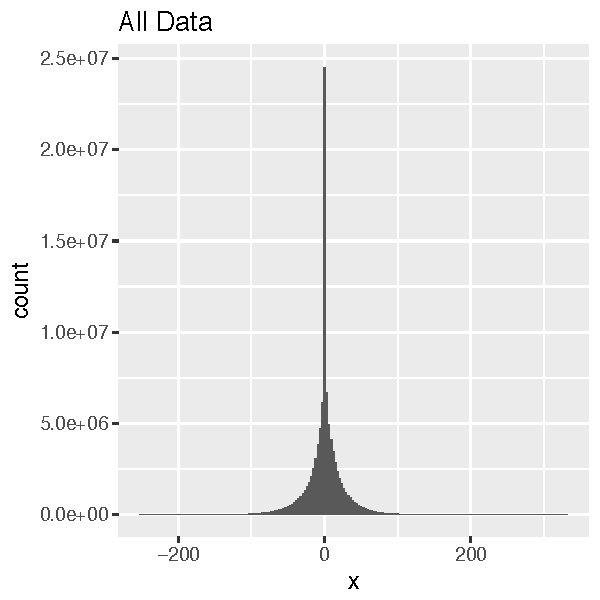
\includegraphics[width=0.16\linewidth]{Figs/raw}
  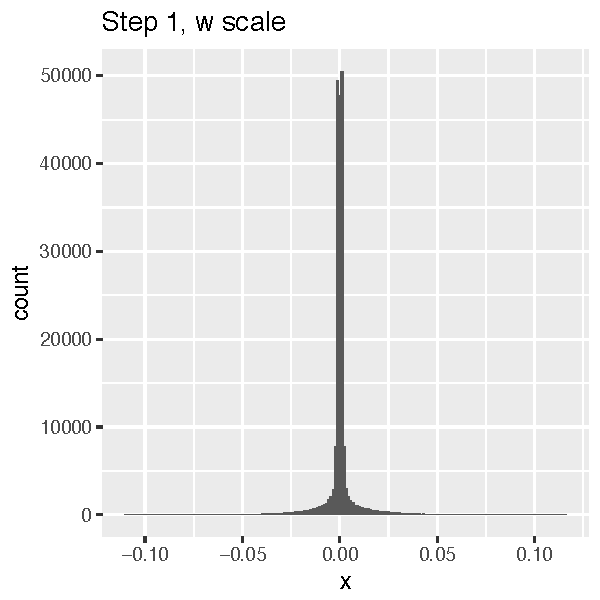
\includegraphics[width=0.16\linewidth]{Figs/raw_1}
  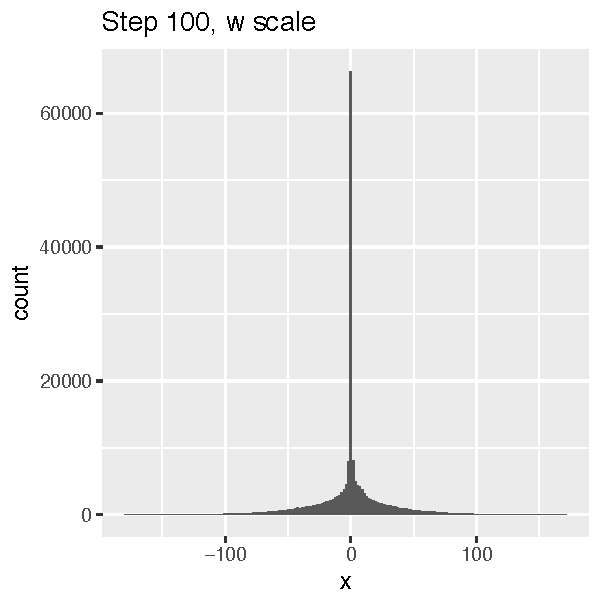
\includegraphics[width=0.16\linewidth]{Figs/raw_100}
  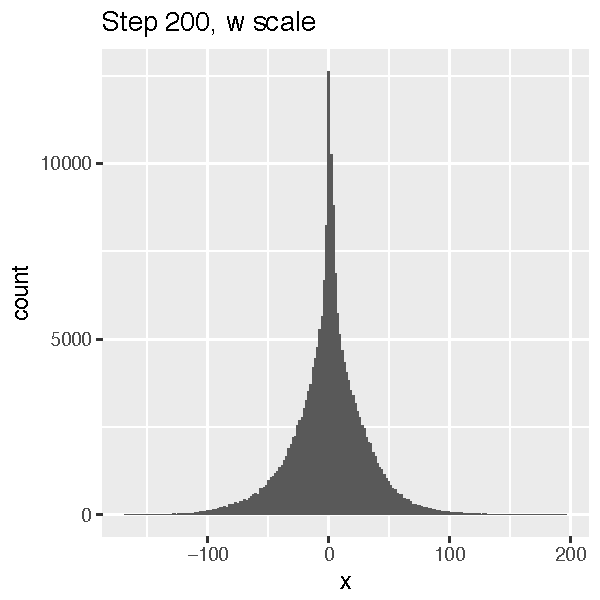
\includegraphics[width=0.16\linewidth]{Figs/raw_200}
  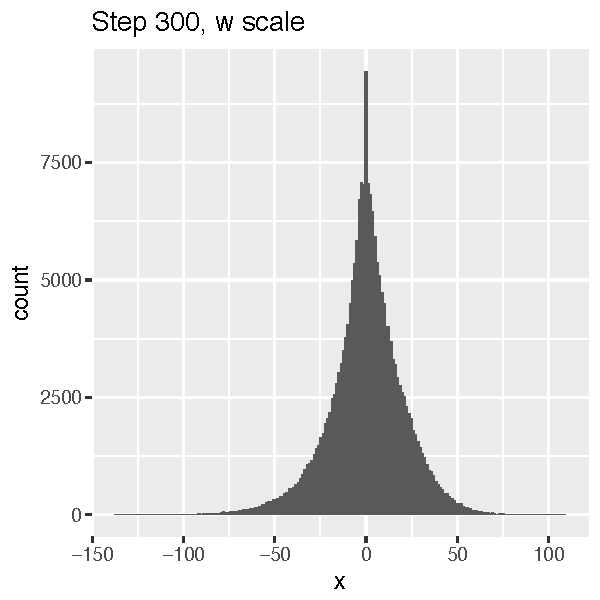
\includegraphics[width=0.16\linewidth]{Figs/raw_300}
  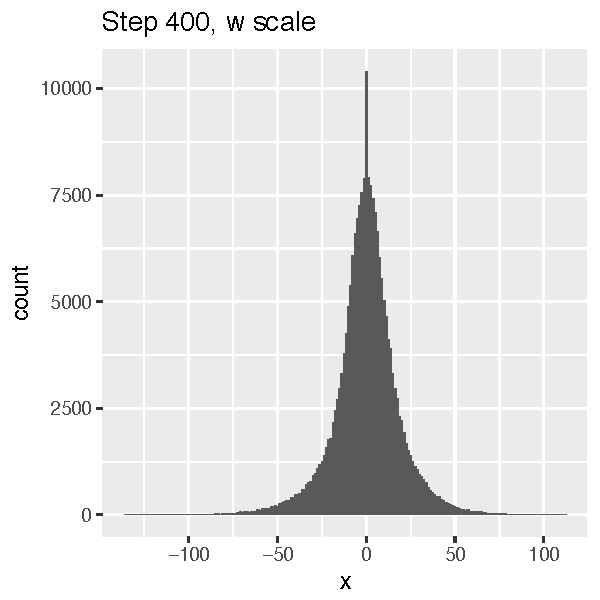
\includegraphics[width=0.16\linewidth]{Figs/raw_400}
  \caption{Histogram of all data followed by a few individual time steps.}
  \label{fig:hist_raw}
\end{figure}

\begin{equation}
  w = sign(x) |x|^{1/5}
\end{equation}

\begin{figure}[!h]
  \centering
  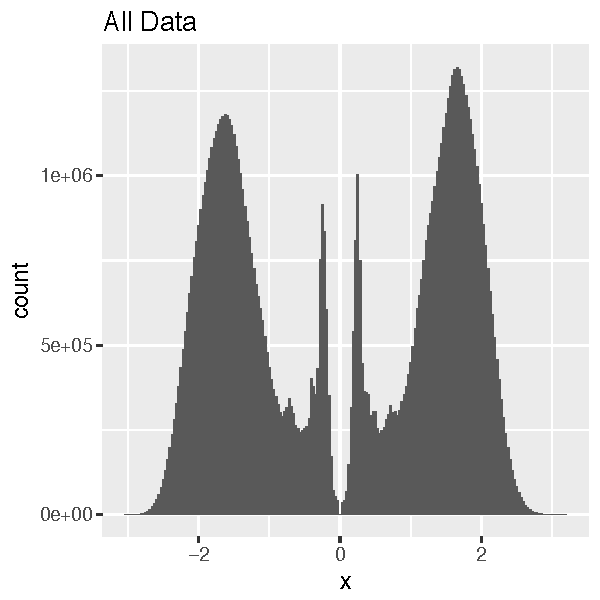
\includegraphics[width=0.16\linewidth]{Figs/tr}
  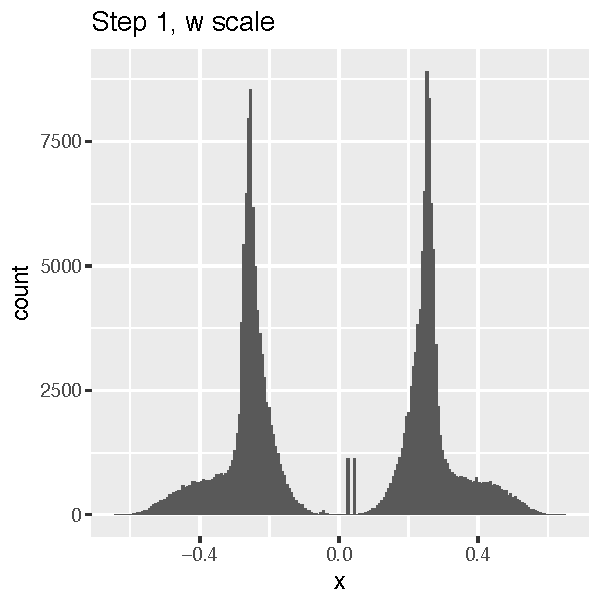
\includegraphics[width=0.16\linewidth]{Figs/tr_1}
  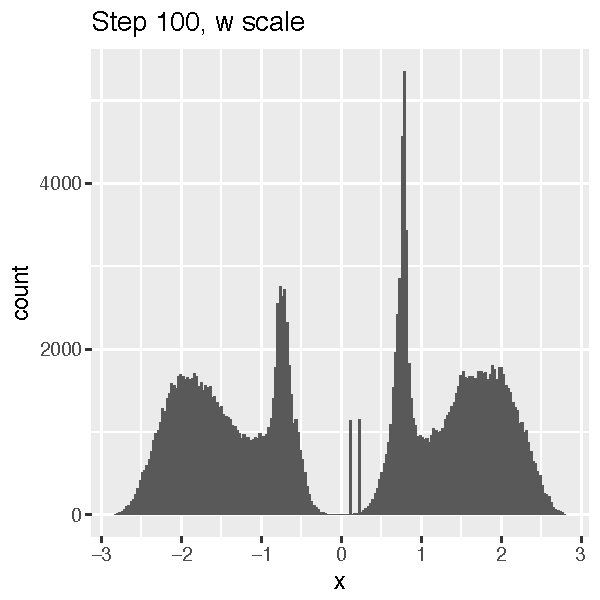
\includegraphics[width=0.16\linewidth]{Figs/tr_100}
  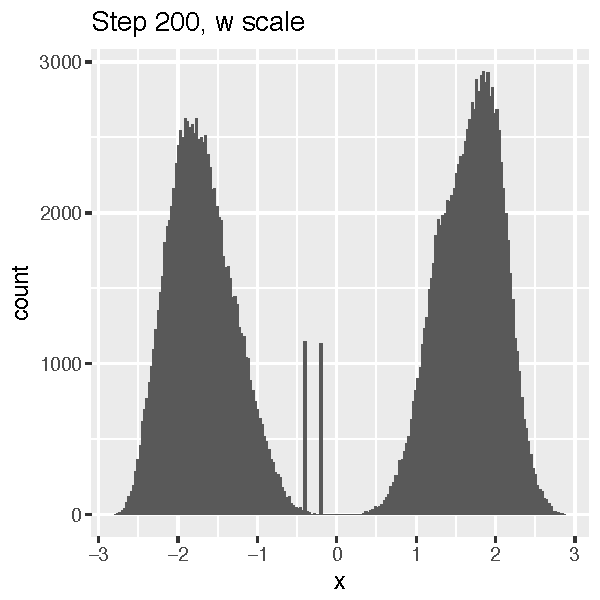
\includegraphics[width=0.16\linewidth]{Figs/tr_200}
  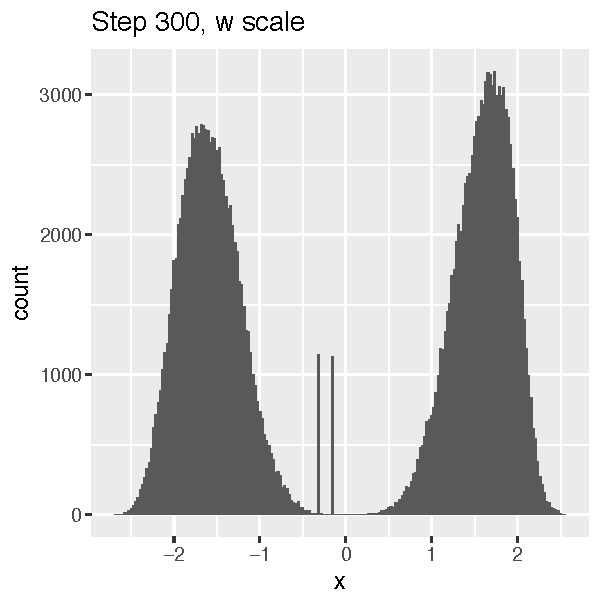
\includegraphics[width=0.16\linewidth]{Figs/tr_300}
  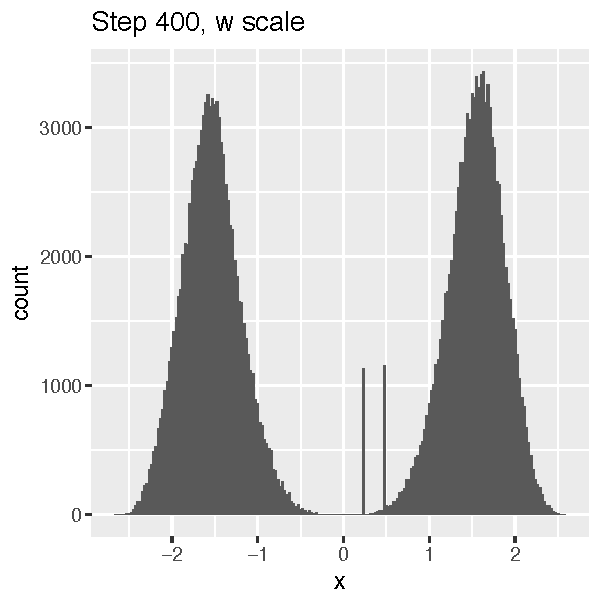
\includegraphics[width=0.16\linewidth]{Figs/tr_400}
  \caption{Same histograms as in Fig.~\ref{fig:hist_raw} after
    removing exact zeroes and transformation to $w$.}
  \label{fig:hist_tr}
\end{figure}

\begin{figure}[!h]
  \centering
  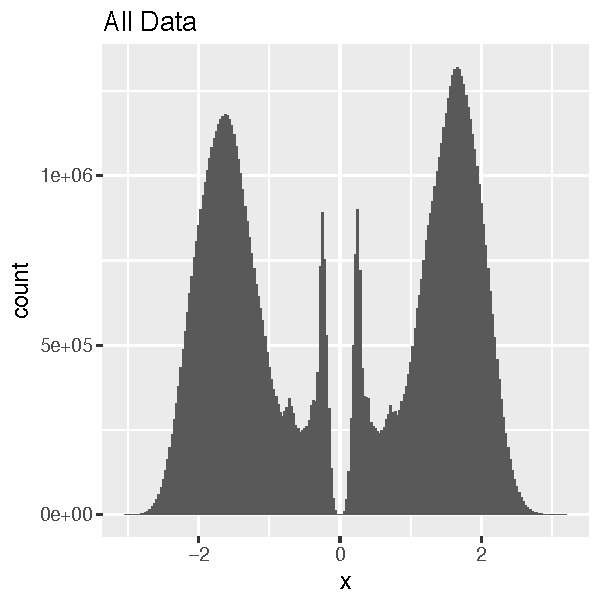
\includegraphics[width=0.16\linewidth]{Figs/trc}
  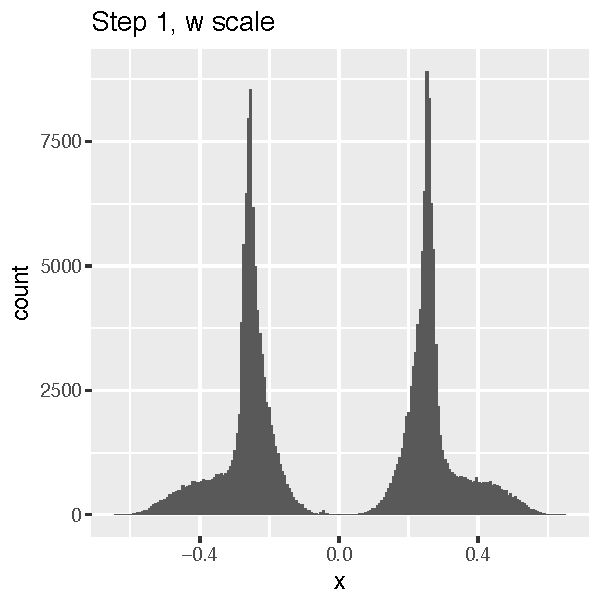
\includegraphics[width=0.16\linewidth]{Figs/trc_1}
  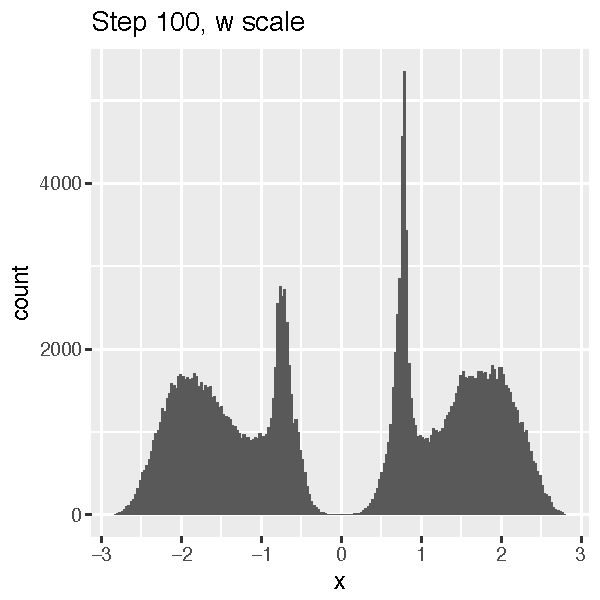
\includegraphics[width=0.16\linewidth]{Figs/trc_100}
  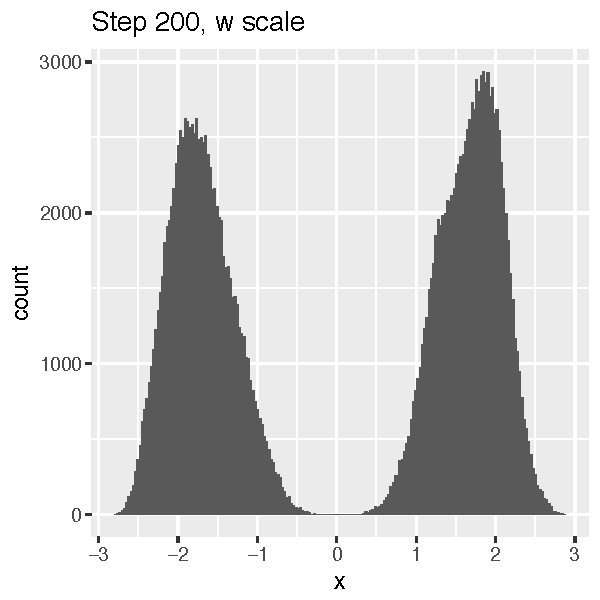
\includegraphics[width=0.16\linewidth]{Figs/trc_200}
  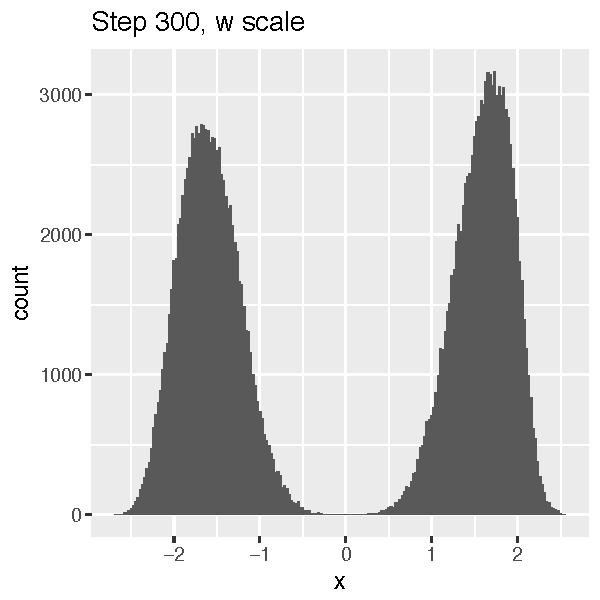
\includegraphics[width=0.16\linewidth]{Figs/trc_300}
  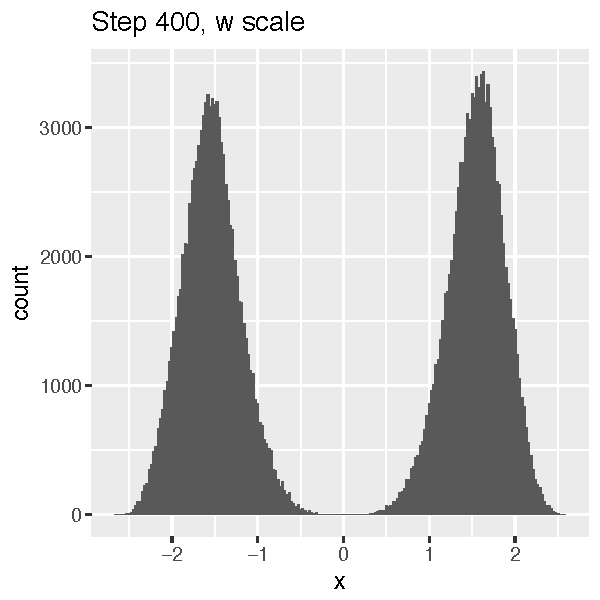
\includegraphics[width=0.16\linewidth]{Figs/trc_400}
  \caption{Same histograms as in Fig.~\ref{fig:hist_tr} after
    removing inlying anomalies.}
  \label{fig:hist_trc}
\end{figure}

